\subsection{Title of work and author and advisor(s) names and affiliations}

The title of the poster is ``Harnessing the Power of Many: Extensible Toolkit 
for Scalable Ensemble Applications''. The author presenting the poster will be 
Vivek Balasubramanian, Electrical and Computer Engineering, Rutgers, the State 
University of New Jersey, under the guidance of Dr. Shantenu Jha and Dr. Matteo
Turilli, Electrical and Computer Engineering, Rutgers, the State University of 
New Jersey.

% Brief description of work being done, including problem being addressed and 
% the research methodology being used

Many scientific problems solved on HPCs consist of applications that rely on the
collective output of multiple tasks as opposed to a single large task. The 
individual tasks within the collection might be uncoupled; if coupled, the tasks
might have global or local synchronizations, and regular or irregular 
communication. This is in contrast to traditional parameter sweeps, or 
high-throughput computing (HTC) applications, where the tasks are typically
identical, uncoupled, idempotent and can be executed in any order.

The execution of an ensemble on HPC machines presents three main challenges: 
(1) encoding scientific problems into algorithms that are amenable to 
distributed and coordinated solution; (2) sizing, acquiring, and managing 
resources for the execution; and (3) managing the execution of the ensemble.

In the absence of generic solutions to these challenges, we designed and 
implemented the Ensemble Toolkit. EnTK adheres to the building blocks 
approach~\cite{} and thus supports coupling with existing runtime systems. 
In addition to extensibility, EnTK enables composability by providing components
specifically to create ensemble-based applications. These features enable EnTK
to overcome flexibility constraints of monolithic workflow systems, and thereby 
support a wide range of application requirements.

EnTK is engineered for scale and diversity of computing platforms and runtime 
systems. EnTK addresses these challenges by decoupling the description of 
ensemble-based applications from their execution into three separate orders of 
concern: specification of task and resource requirements; resource selection and
acquisition; and task execution management.

\subsection{Abstract of results to be presented in poster}

We present three sets of results in the poster. We first present the performance
benchmark of an EnTK prototype that provide a reference hardware configuration 
to support execution of up to $O(10^6)$ tasks. In the second set of results, we
present the weak and strong scaling behavior of EnTK. Lastly, we implement and 
execute at scale our two use cases, seismic inversion and adaptive analog 
workflow.

We prototyped EnTK instantiating only multiple producers and consumers of tasks.
The producers push into RabbitMQ queues and consumers pull from these queues.
With a total of $10^6$ tasks, we benchmark the prototype to observe the total
execution time, base and peak memory consumption as a function of the number of
producers, consumers and queues.

\begin{figure} 
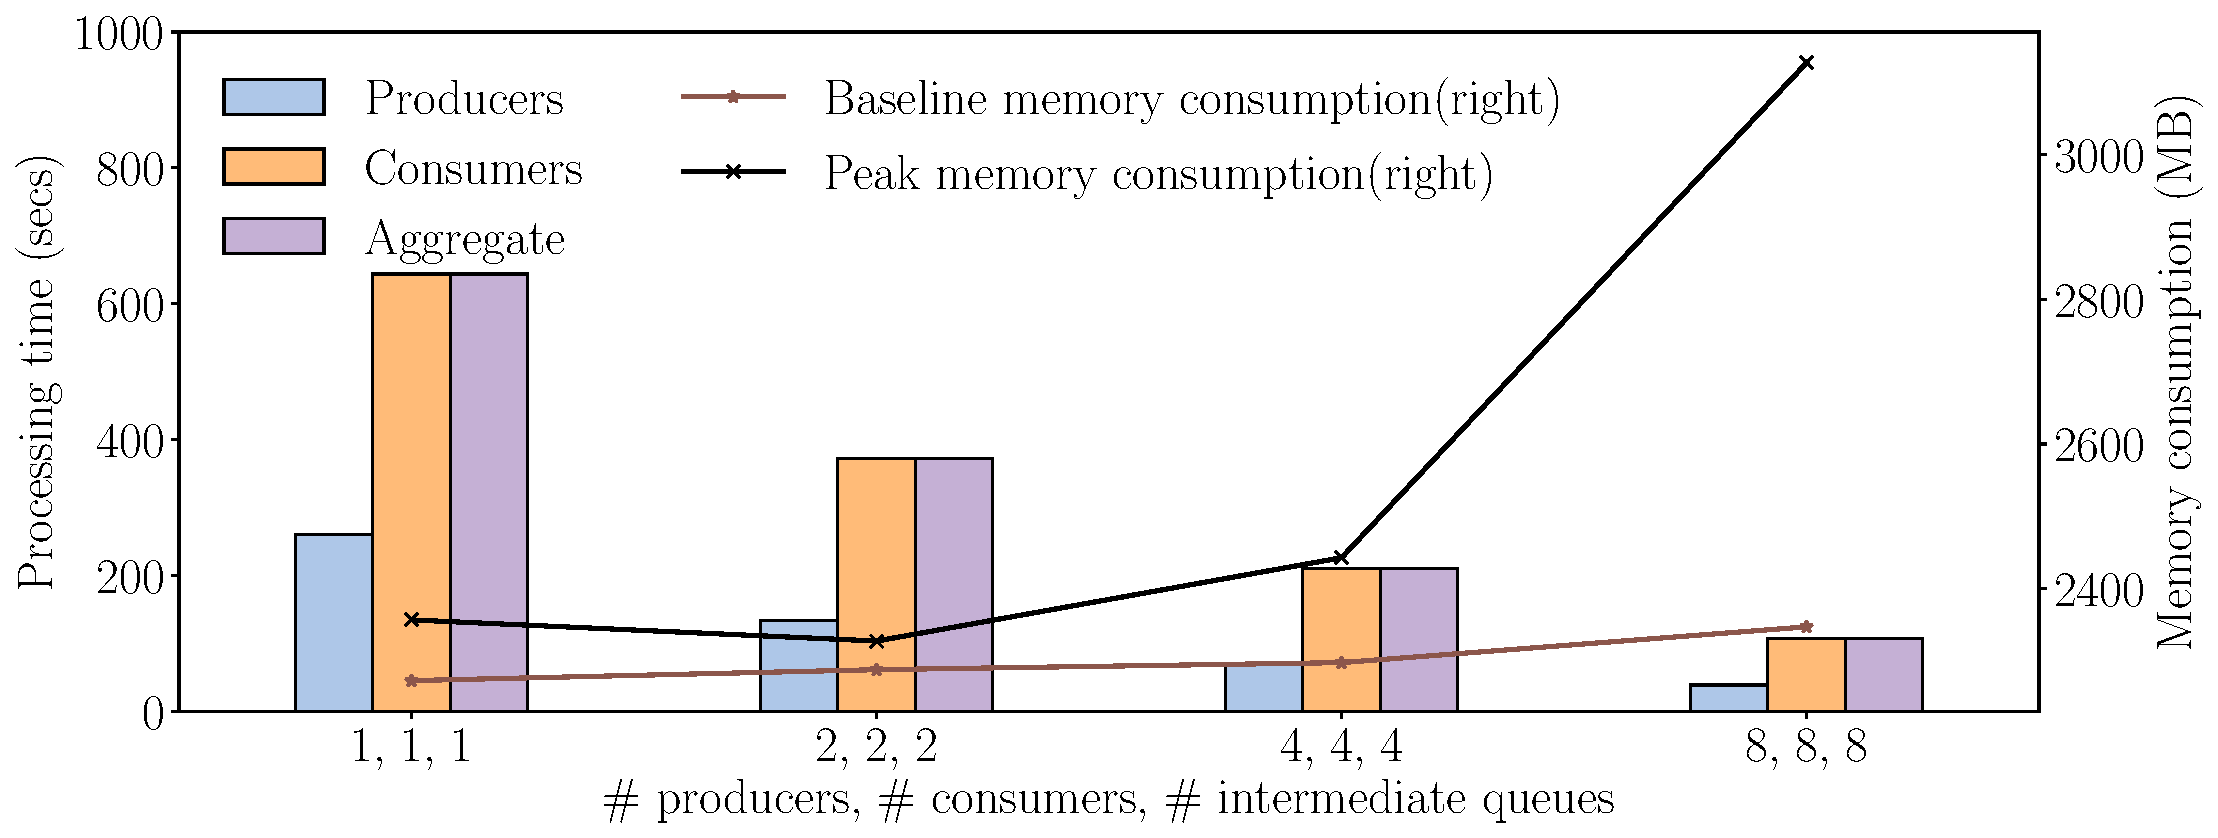
\includegraphics[width=0.48\textwidth]{figs/prototype.pdf}
\caption{EnTK prototype}\label{fig:prototype}
\end{figure}

In Figure~\ref{fig:prototype}, we show that the execution duration decreases
linearly at the cost of increased memory usage. We also gather from the 
benchmark that EnTK can be tuned, by varying the number of producers, consumers 
and queues, depending on the resource and application requirements.


Next we present experiments to characterize weak and strong scalability of EnTK.
Weak scaling experiments describe the performance of EnTK when supporting 
varying levels of concurrency; Strong scaling experiments describe the 
performance of EnTK when executing a workload larger than the amount of 
available resources. For the purposes of the poster, we focus only on the Task
Execution Time and the EnTK Management Overhead. The remaining durations are
a function of the Python language or the underlying RTS. Enhancements to these
will directly reflect improvements in these durations and thus we consider them
out of scope.

In the case of weak scaling, we run four applications each with 1 pipeline, 1 
stage per pipeline, 512, 1024, 2048 and 4096 tasks per stage and number of cores
proportional to the number of tasks in the stage. While in the case of strong 
scaling, we run three applications each with 1 pipeline, 1 stage per pipeline, 
8192 tasks per stage and 1024, 2048 and 4096 cores. Each task, configured to
run on 1 core for \(\approx\)600 seconds, executes a Gromacs simulation. Each 
task requires an input of 4 files with an aggregate size of 550KB.
\begin{figure} 
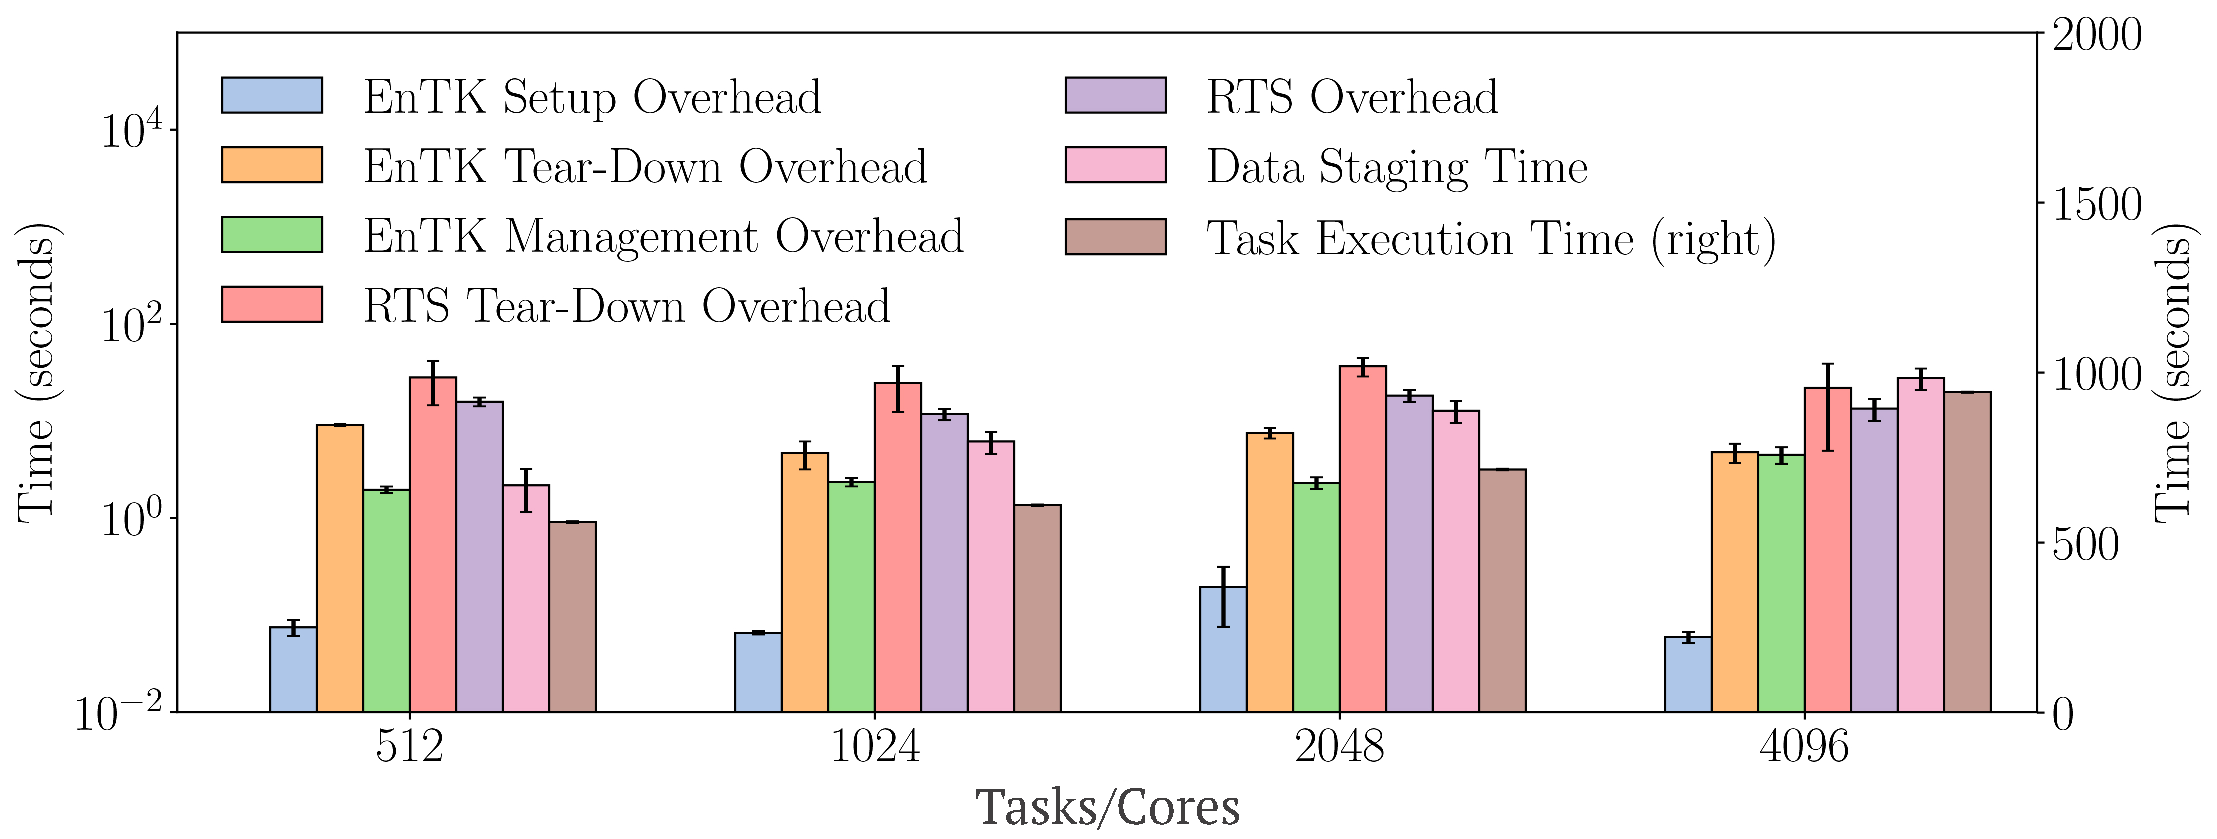
\includegraphics[width=0.48\textwidth]{figs/weak_scaling_titan_orte_reduced.pdf}
\caption{Weak scaling}\label{fig:weak_scaling}
\end{figure}

In Figure~\ref{fig:weak_scaling}, the Task Execution Time increases even though
there are sufficient resources to run all the tasks. We attribute this to the
limitations in the current implementation of the RTS and the ORTE distributed 
virtual machine of OpenMP. EnTK Management Overhead remains constant up to 2048
above which the number of tasks strain the resources leading to an increase in
the overhead. The Data Staging Duration increases since the total amount of 
data increases with increase in the number of tasks.

\begin{figure} 
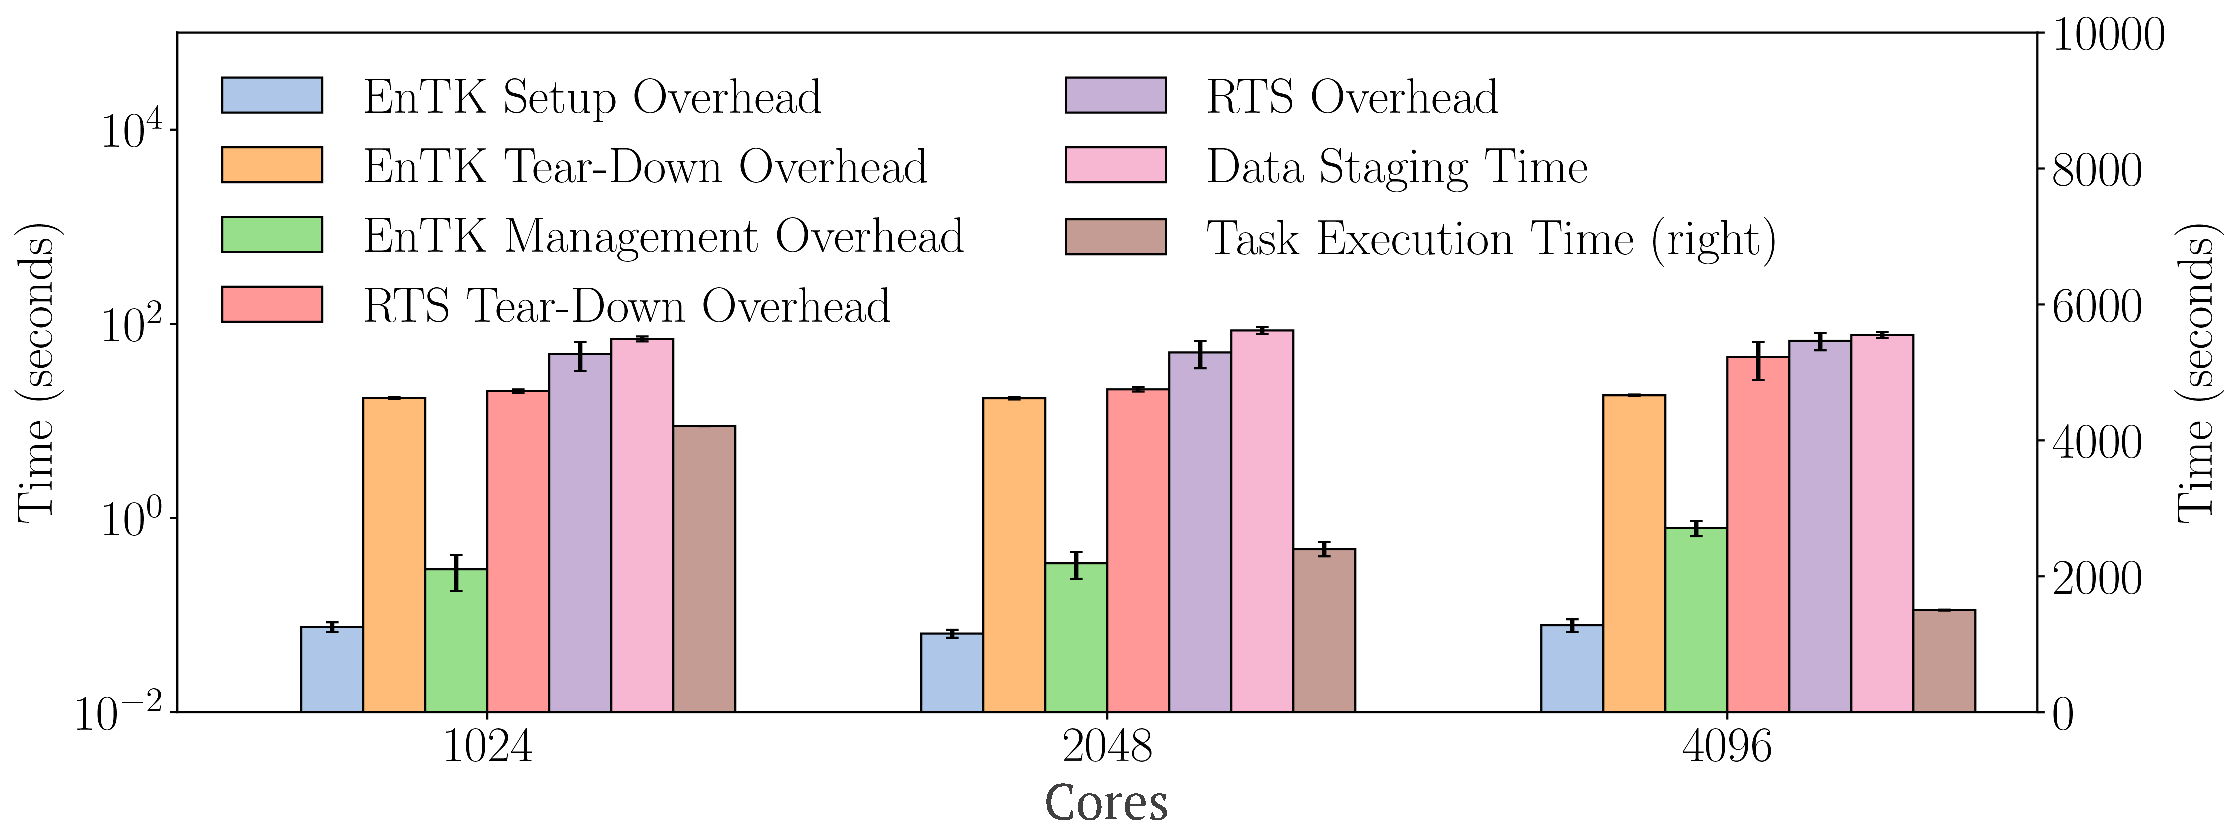
\includegraphics[width=0.48\textwidth]{figs/strong_scaling_titan_orte.pdf}
\caption{Strong scaling}\label{fig:strong_scaling}
\end{figure}

In Figure~\ref{fig:strong_scaling}, the Task Execution Time reduces linearly 
with an increase in the number of available cores. EnTK Management Overhead 
remains constant at \(\approx\)8 seconds and Data Staging Duration remains 
constant at \(\approx\)90 seconds since the total number of tasks remains
constant and thus the total data staged is also constant.


We use EnTK to encode the forward simulations of the seismic tomography 
workflow. These simulations account for more than 90\% of the computation time 
of the workflow, requiring 384 nodes for each earthquake simulation, and 40MB
of input data each. Concurrent simulation of earthquakes incur a high failure 
rate and are resubmitted automatically by EnTK.

\begin{figure} 
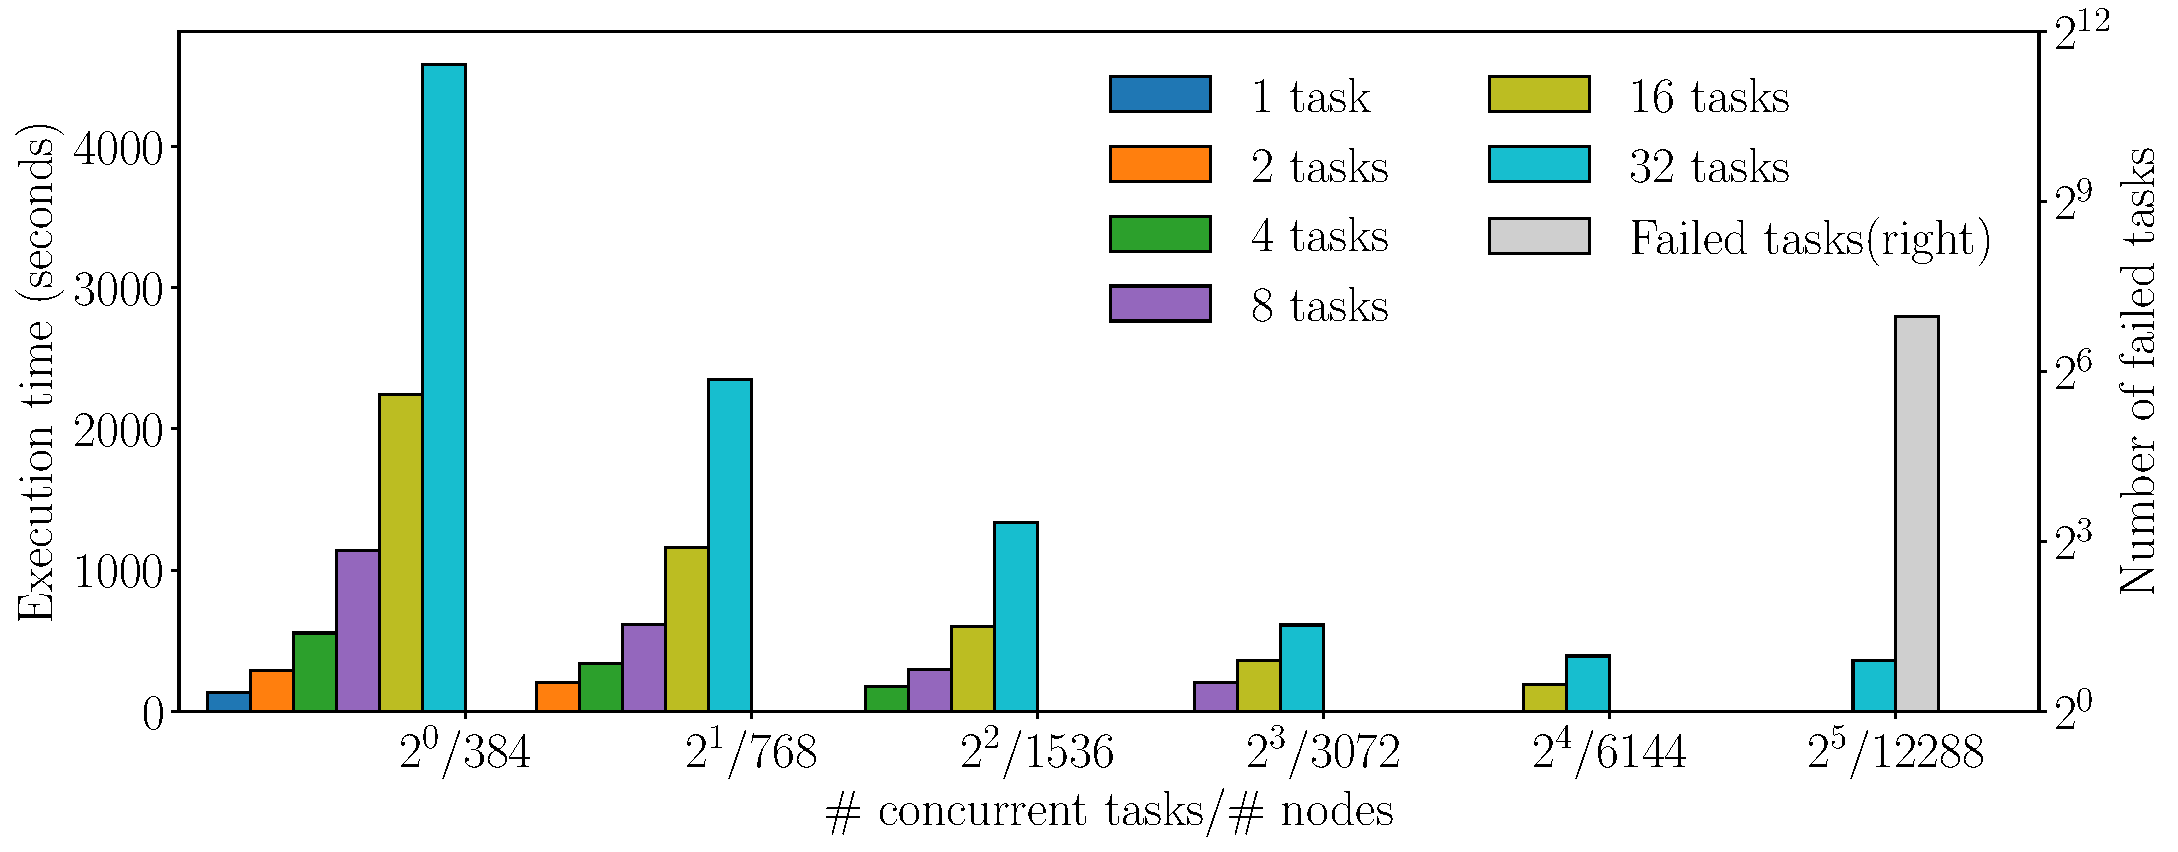
\includegraphics[width=0.48\textwidth]{figs/specfem_exec_time_varying_concurrency_titan.pdf}
\caption{Specfem execution time and failure rate}\label{fig:specfem}
\end{figure}

In Figure~\ref{fig:specfem}, we run six applications with 1 pipeline, 1 stage 
per pipeline and 1, 2, 4, 8, 16 and 32 tasks per stage. Each of the applications
is run at different levels of concurrency. We observe that for constant
concurrency, the execution time increases linearly with increase in the number 
of tasks and the execution time reduces linearly when increasing the 
concurrency. We also observe that reducing concurrency eliminates failures: we 
encountered no failures in executions with up to $O(2^4)$ concurrent tasks and 
6,144 nodes. At $O(2^5)$ concurrent tasks and 12,288 nodes, 157 tasks failed. 
EnTK automatically submits a failed tasks and as a result we observed a Task 
Execution Time of \(\approx\)360 seconds.


We use EnTK to implement the AUA algorithm to iteratively and dynamically 
identify locations of the analogs. We perform experiments to compare our 
implementation with the status quo method, i.e. random selection of locations, 
and observe the speedup of the proposed algorithm.

\begin{figure} 
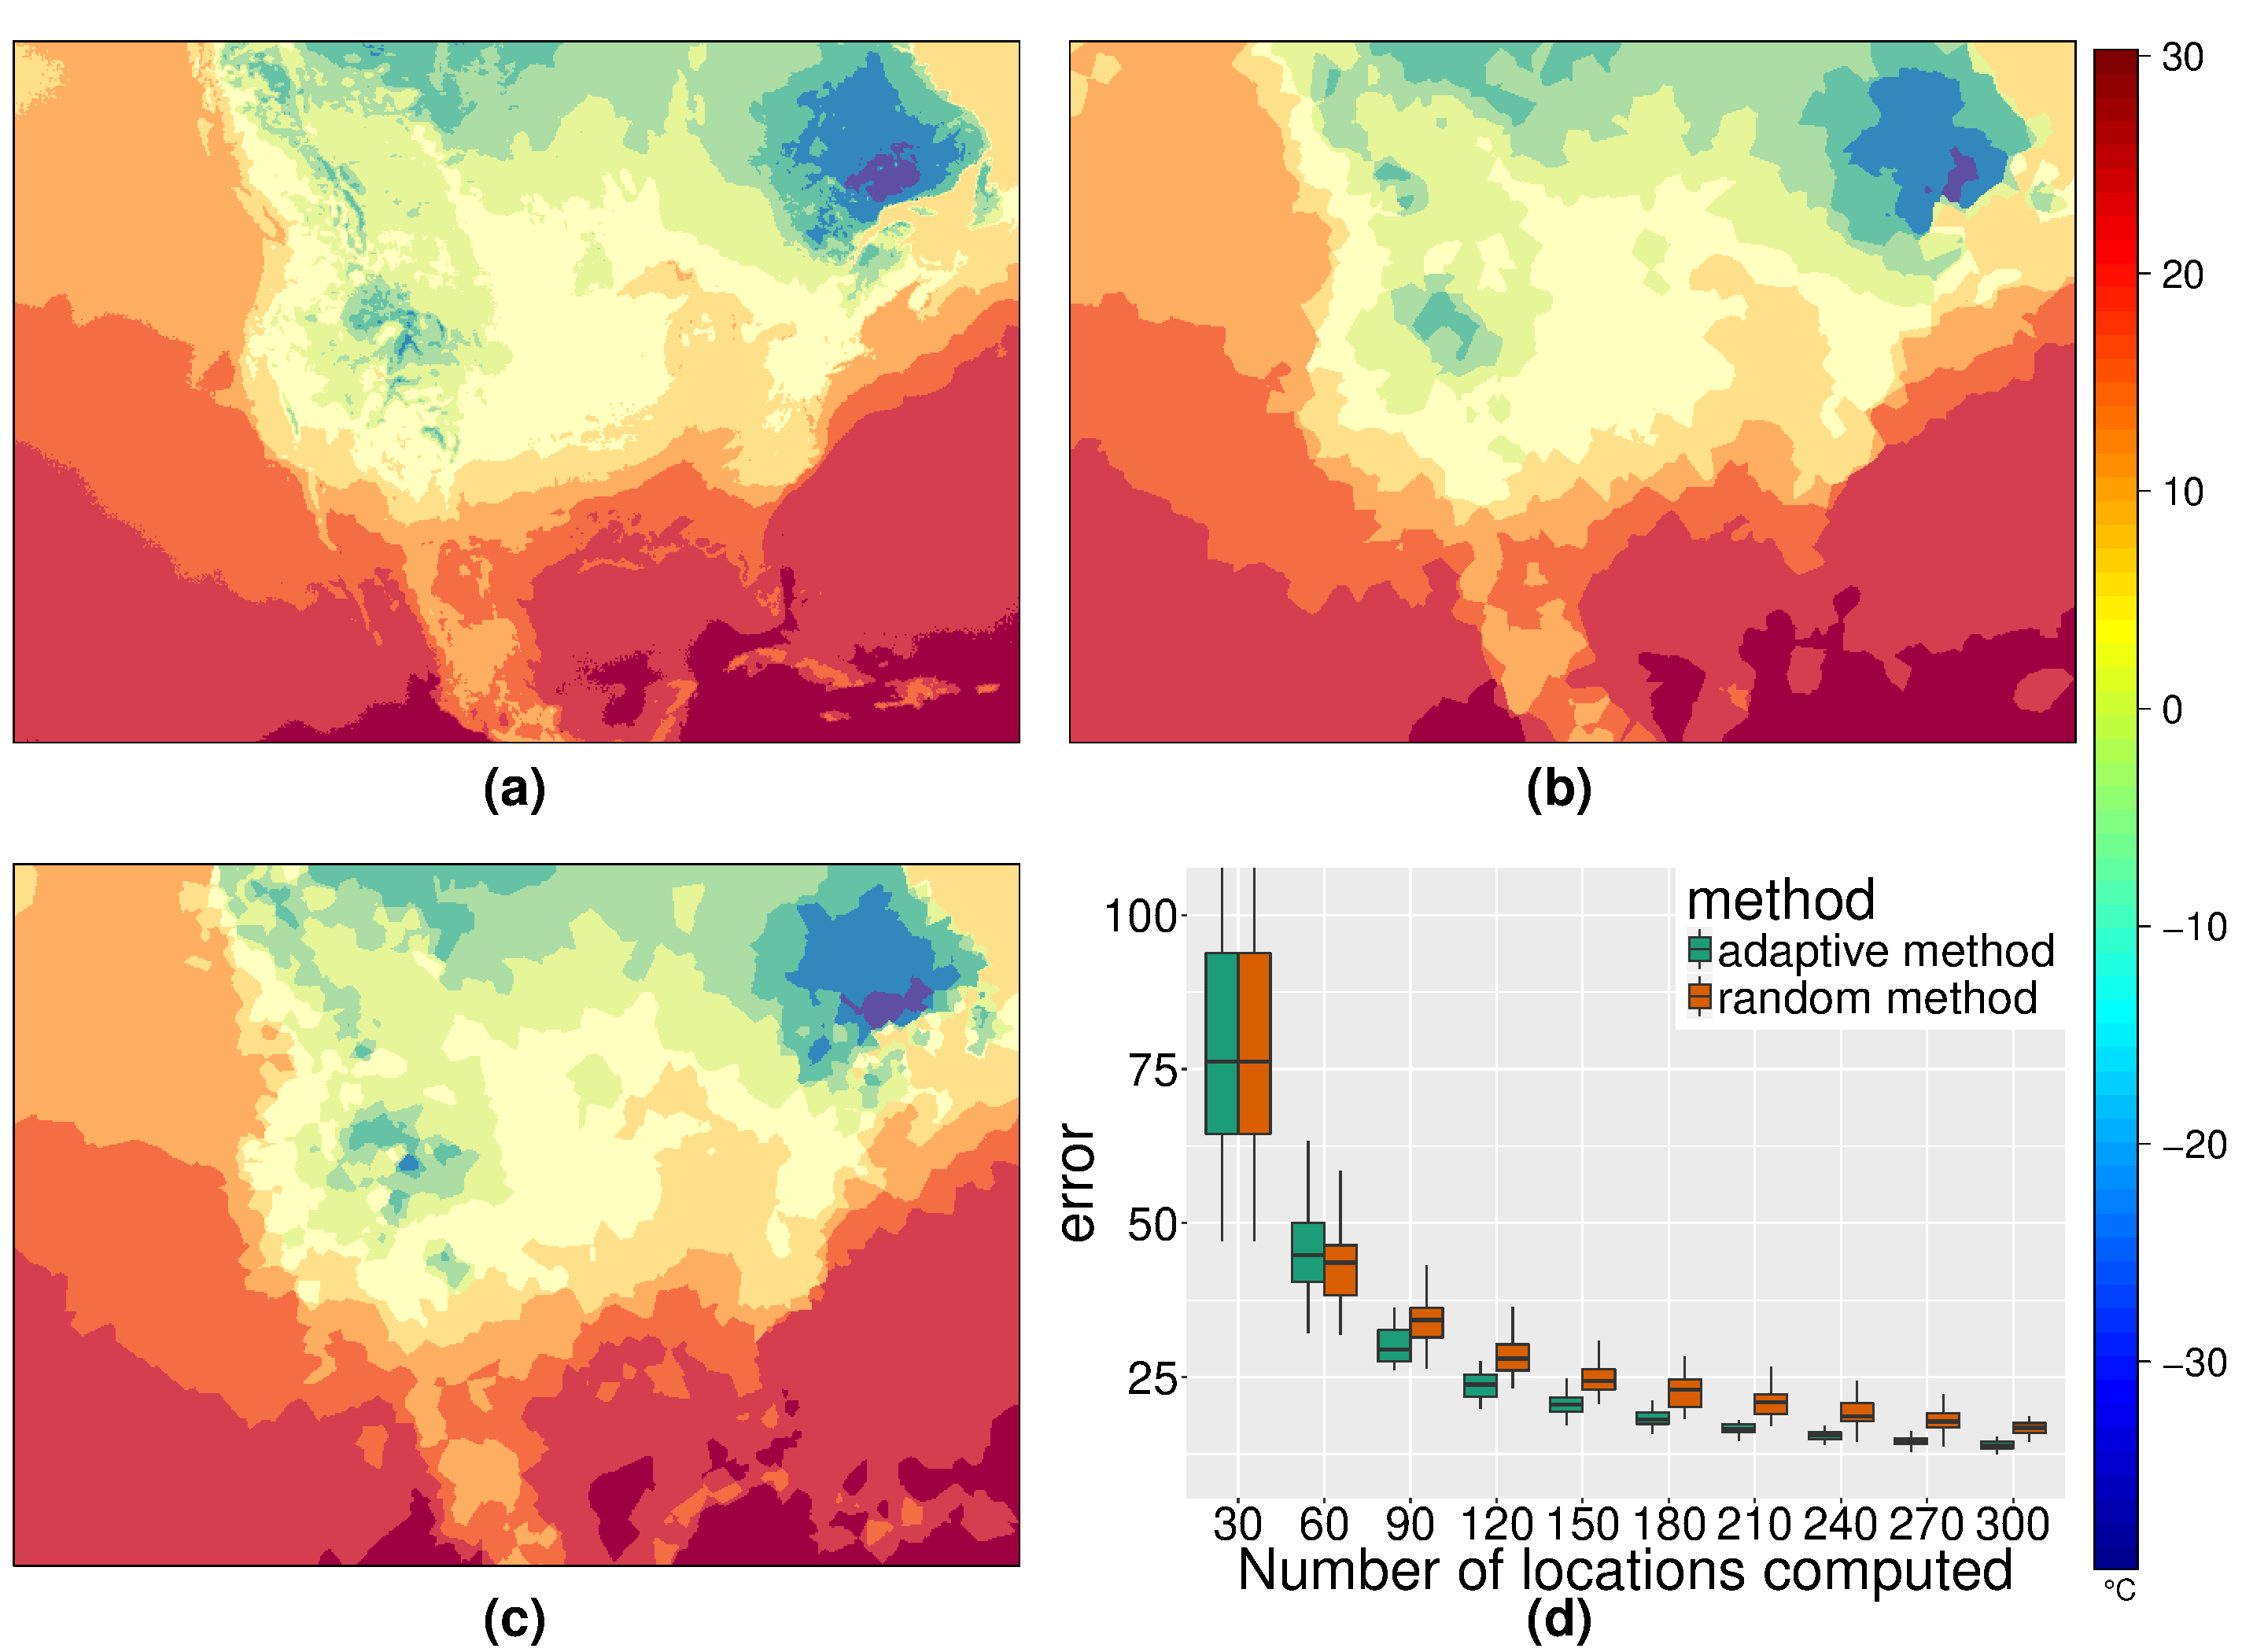
\includegraphics[width=0.48\textwidth]{figs/EX_PSU_error_plot_2x2.pdf}
\caption{Error in Analog Ensemble execution}\label{fig:anen}
\end{figure}

Figure~\ref{fig:anen} shows the prediction maps and errors obtained from the two
implementations. The AUA algorithm generates a map (b, c) with certain 
areas that have a better representation of the analysis than the map generated 
by a random selection of pixels. Box plot (d) shows that the error converges 
faster in the AUA algorithm than in the random selection.